\begin{center}

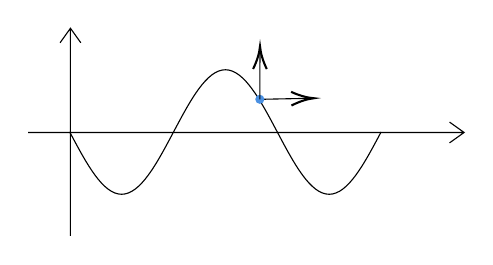
\begin{tikzpicture}[x=0.75pt,y=0.75pt,yscale=-1,xscale=1]
%uncomment if require: \path (0,300); %set diagram left start at 0, and has height of 300

%Shape: Axis 2D [id:dp17044305030121132] 
\draw  (70,150.23) -- (280,150.23)(90.34,100) -- (90.34,200) (273,145.23) -- (280,150.23) -- (273,155.23) (85.34,107) -- (90.34,100) -- (95.34,107)  ;
%Shape: Wave [id:dp3213186683813747] 
\draw   (90,150) .. controls (98.15,165.37) and (105.95,180) .. (115,180) .. controls (124.05,180) and (131.85,165.37) .. (140,150) .. controls (148.15,134.63) and (155.95,120) .. (165,120) .. controls (174.05,120) and (181.85,134.63) .. (190,150) .. controls (198.15,165.37) and (205.95,180) .. (215,180) .. controls (224.05,180) and (231.85,165.37) .. (240,150) ;
%Straight Lines [id:da4960855789495031] 
\draw    (181.58,134.25) -- (205.67,133.77) ;
\draw [shift={(207.67,133.73)}, rotate = 178.86] [color={rgb, 255:red, 0; green, 0; blue, 0 }  ][line width=0.75]    (10.93,-3.29) .. controls (6.95,-1.4) and (3.31,-0.3) .. (0,0) .. controls (3.31,0.3) and (6.95,1.4) .. (10.93,3.29)   ;
%Shape: Circle [id:dp4675822922340589] 
\draw  [color={rgb, 255:red, 74; green, 144; blue, 226 }  ,draw opacity=1 ][fill={rgb, 255:red, 74; green, 144; blue, 226 }  ,fill opacity=1 ] (179.67,134.25) .. controls (179.67,133.19) and (180.52,132.33) .. (181.58,132.33) .. controls (182.64,132.33) and (183.49,133.19) .. (183.49,134.25) .. controls (183.49,135.3) and (182.64,136.16) .. (181.58,136.16) .. controls (180.52,136.16) and (179.67,135.3) .. (179.67,134.25) -- cycle ;
%Straight Lines [id:da7406502193343325] 
\draw    (181.58,134.25) -- (181.66,110.73) ;
\draw [shift={(181.67,108.73)}, rotate = 90.2] [color={rgb, 255:red, 0; green, 0; blue, 0 }  ][line width=0.75]    (10.93,-3.29) .. controls (6.95,-1.4) and (3.31,-0.3) .. (0,0) .. controls (3.31,0.3) and (6.95,1.4) .. (10.93,3.29)   ;

\end{tikzpicture}

\end{center}